\section{Arquitectura del compilador}
\label{sec:compiler-architecture}

Los compiladores son programas que transforman el código fuente escrito en un lenguaje en
otro lenguaje, normalmente código máquina. Un compilador toma un programa en un lenguaje,
el \emph{lenguaje fuente}, y lo traduce a un programa equivalente en otro lenguaje, el \emph{lenguaje de
destino}.

Para lograrlo, los compiladores suelen tener una serie de fases o pases que se ejecutan en
secuencia. El objetivo de estos pases es traducir el código de alto nivel en código de bajo nivel
que la máquina pueda ejecutar. Tras cada pasada, el código se acerca cada vez más a la
representación final. Estas fases están hoy en día bien definidas y diferentes compiladores las
implementan en alguna forma u otra \cite[Chap. 1.2]{aho2014compilers}.

La primera pasada de un compilador típico es la fase de \textbf{análisis léxico (\textit{lexical analysis})}.
En esta fase, el código fuente se descompone en un flujo de tokens, cada uno de los cuales representa una única pieza
del código. El analizador léxico (\emph{lexer}) identifica palabras clave, identificadores, literales y otros
tokens que forman los bloques de construcción del código fuente.

La siguiente pasada es la fase de \textbf{análisis sintáctico (\textit{syntax analysis})}, también conocida como fase del
\textit{parser}. En esta fase, los tokens producidos por el \emph{lexer} se analizan según las
reglas de la gramática del lenguaje de programación. El analizador sintáctico construye un
\emph{parse tree} o un árbol sintáctico abstracto (\acrfull{AST}) que representa la estructura del
código.

La tercera pasada es la fase de \textbf{análisis semántico (\textit{semantic analysis})}, en la que el compilador comprueba la
correctitud semántica del código, como la comprobación de errores de tipo, variables no
definidas y operaciones no válidas. El analizador semántico (\emph{semantic analyzer}) construye una tabla de símbolos
que contiene información sobre las variables, funciones y otras entidades definidas en el
código.

La cuarta pasada es la fase de \textbf{generación de código (\textit{code generation})}. El compilador toma el \acrshort{AST} y la tabla de
símbolos producidos por las fases anteriores y genera código de bajo nivel que puede ser
ejecutado por la máquina. El generador de código suele generar código en lenguaje
ensamblador o código máquina. En otros casos, genera bytecode, como en Java o cuando se
utiliza el compilador \acrfull{JIT} de Python.

Finalmente, puede haber cero o más fases de \textbf{optimización del código (\textit{code optimization})}.
Estas son, desde un punto de vista teórico, opcionales, pero suelen incluirse por defecto en los compiladores
modernos. En esta fase, el compilador analiza el código generado e intenta mejorar su
eficiencia aplicando diversas técnicas de optimización. Algunos ejemplos de optimizaciones
son:

\begin{itemize}
    \item plegado de constantes (\textit{constant folding}) \cite[Chap. 8.5.4]{aho2014compilers},
    \item desenrollado de bucles (\textit{loop unrolling}) \cite[Chap. 10.5]{aho2014compilers},
    \item asignación de registros (\textit{register allocation}) \cite[Chap. 8.1.4]{aho2014compilers},
    \item propagación de constantes (\textit{constant propagation}) \cite[Chap. 9]{aho2014compilers},
    \item análisis de vida útil (\textit{livenes analysis}) \cite[Chap. 9]{aho2014compilers},
    \item y muchos más\ldots
\end{itemize}

Las optimizaciones \emph{locales} de código se refieren a mejoras dentro de un bloque básico, mientras
que la optimización \emph{global} de código es cuando las mejoras tienen en cuenta
lo que ocurre más allá de un bloque básico.
En Rust, un ejemplo de optimización global es la optimización
del tiempo de enlace (\acrfull{LTO}) \cite{huss2020}.

La Fig. \ref{fig:compiler-phases} tomada de \cite{aho2014compilers} visualiza intuitivamente
las fases del compilador descritas en esta sección.

\begin{figure}[!htb]
    \centering
    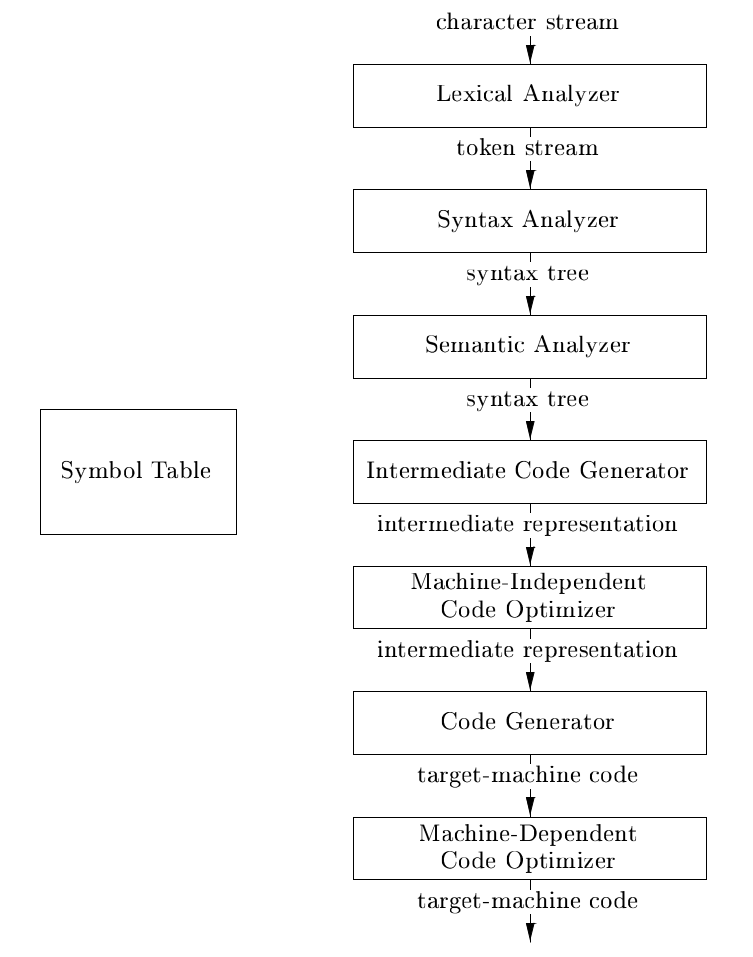
\includegraphics[scale=0.40]{compiler-phases.png}
    \caption{Fases de un compilador.}
    \label{fig:compiler-phases}
\end{figure}

En la práctica, las fases pueden tener límites poco claros. Pueden solaparse y algunas pueden
saltarse por completo. En secciones posteriores estudiaremos la arquitectura del compilador de
Rust \emph{rustc} y explicaremos su arquitectura en términos generales.